\documentclass{minimal}
\usepackage{graphicx,color}
\usepackage[utf8]{inputenc}
\usepackage[papersize={419.00bp,332.00bp},text={419.00bp,332.00bp}]{geometry}
\begin{document}
\centering
% Title: gl2ps_renderer figure
% Creator: GL2PS 1.4.2, (C) 1999-2020 C. Geuzaine
% For: Octave
% CreationDate: Mon Dec 12 16:54:16 2022
\setlength{\unitlength}{1pt}
\begin{picture}(0,0)
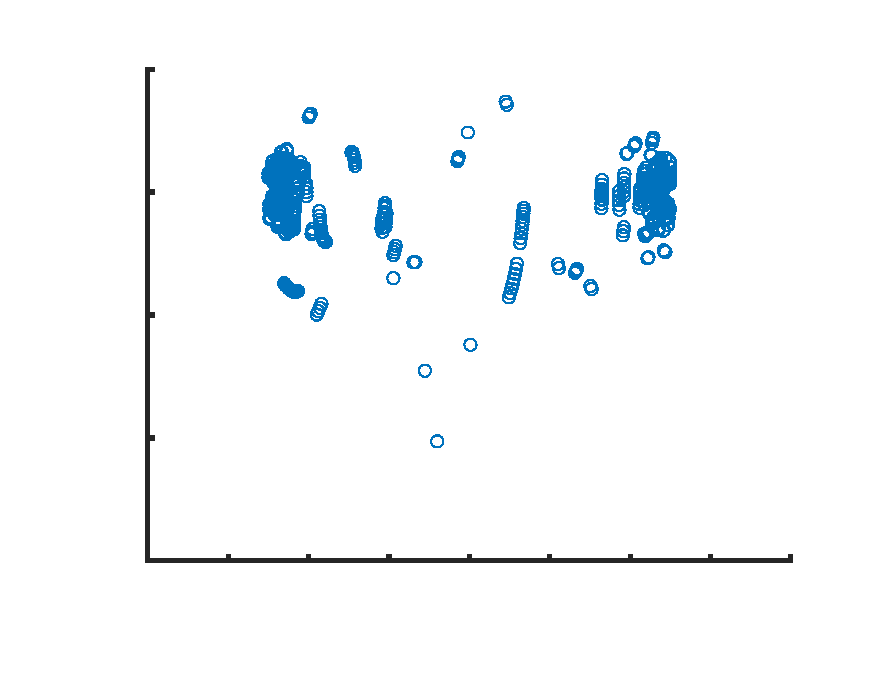
\includegraphics[scale=1]{DoubleKapitzaPoincareMapped-inc}
\end{picture}%
\begin{picture}(419,332)(0,0)
\fontsize{22}{0}\selectfont\put(70.9854,46.4376){\makebox(0,0)[t]{\textcolor[rgb]{0.15,0.15,0.15}{{-0.8}}}}
\fontsize{22}{0}\selectfont\put(109.562,46.4376){\makebox(0,0)[t]{\textcolor[rgb]{0.15,0.15,0.15}{{-0.6}}}}
\fontsize{22}{0}\selectfont\put(148.139,46.4376){\makebox(0,0)[t]{\textcolor[rgb]{0.15,0.15,0.15}{{-0.4}}}}
\fontsize{22}{0}\selectfont\put(186.716,46.4376){\makebox(0,0)[t]{\textcolor[rgb]{0.15,0.15,0.15}{{-0.2}}}}
\fontsize{22}{0}\selectfont\put(225.293,46.4376){\makebox(0,0)[t]{\textcolor[rgb]{0.15,0.15,0.15}{{0}}}}
\fontsize{22}{0}\selectfont\put(263.87,46.4376){\makebox(0,0)[t]{\textcolor[rgb]{0.15,0.15,0.15}{{0.2}}}}
\fontsize{22}{0}\selectfont\put(302.447,46.4376){\makebox(0,0)[t]{\textcolor[rgb]{0.15,0.15,0.15}{{0.4}}}}
\fontsize{22}{0}\selectfont\put(341.024,46.4376){\makebox(0,0)[t]{\textcolor[rgb]{0.15,0.15,0.15}{{0.6}}}}
\fontsize{22}{0}\selectfont\put(379.601,46.4376){\makebox(0,0)[t]{\textcolor[rgb]{0.15,0.15,0.15}{{0.8}}}}
\fontsize{22}{0}\selectfont\put(59.9991,62.9417){\makebox(0,0)[r]{\textcolor[rgb]{0.15,0.15,0.15}{{-15}}}}
\fontsize{22}{0}\selectfont\put(59.9991,121.956){\makebox(0,0)[r]{\textcolor[rgb]{0.15,0.15,0.15}{{-10}}}}
\fontsize{22}{0}\selectfont\put(59.9991,180.971){\makebox(0,0)[r]{\textcolor[rgb]{0.15,0.15,0.15}{{-5}}}}
\fontsize{22}{0}\selectfont\put(59.9991,239.985){\makebox(0,0)[r]{\textcolor[rgb]{0.15,0.15,0.15}{{0}}}}
\fontsize{22}{0}\selectfont\put(59.9991,299){\makebox(0,0)[r]{\textcolor[rgb]{0.15,0.15,0.15}{{5}}}}
\fontsize{24}{0}\selectfont\put(225.293,24.4376){\makebox(0,0)[t]{\textcolor[rgb]{0.15,0.15,0.15}{{$\theta_2/(2 \pi)$}}}}
\fontsize{24}{0}\selectfont\put(23.9991,180.971){\rotatebox{90}{\makebox(0,0)[b]{\textcolor[rgb]{0.15,0.15,0.15}{{$\omega_2$}}}}}
\fontsize{24}{0}\selectfont\put(225.293,309){\makebox(0,0)[b]{\textcolor[rgb]{0,0,0}{{Poincaré Section at $\theta_1 = 0$}}}}
\end{picture}
\end{document}
